\documentclass{article}

\usepackage{lastpage} % for the number of the last page in the document
\usepackage{fancyhdr}
\usepackage{geometry}
\usepackage{graphicx}
\usepackage{grffile}
\usepackage[utf8x]{inputenc}
\geometry{a4paper}
\geometry{portrait}
\pagestyle{fancy}
\fancyhf{}
\lhead{User Manual KinderFinder}
\rhead{Section \thesection}
\lfoot{}
\rfoot{Page \thepage\ of \pageref{LastPage}}





\begin{document}
\tableofcontents
\newpage


\section{Welcome to KinderFinder}
\subsection{What is KinderFinder}



%\begin{figure}[H]
%\centering
%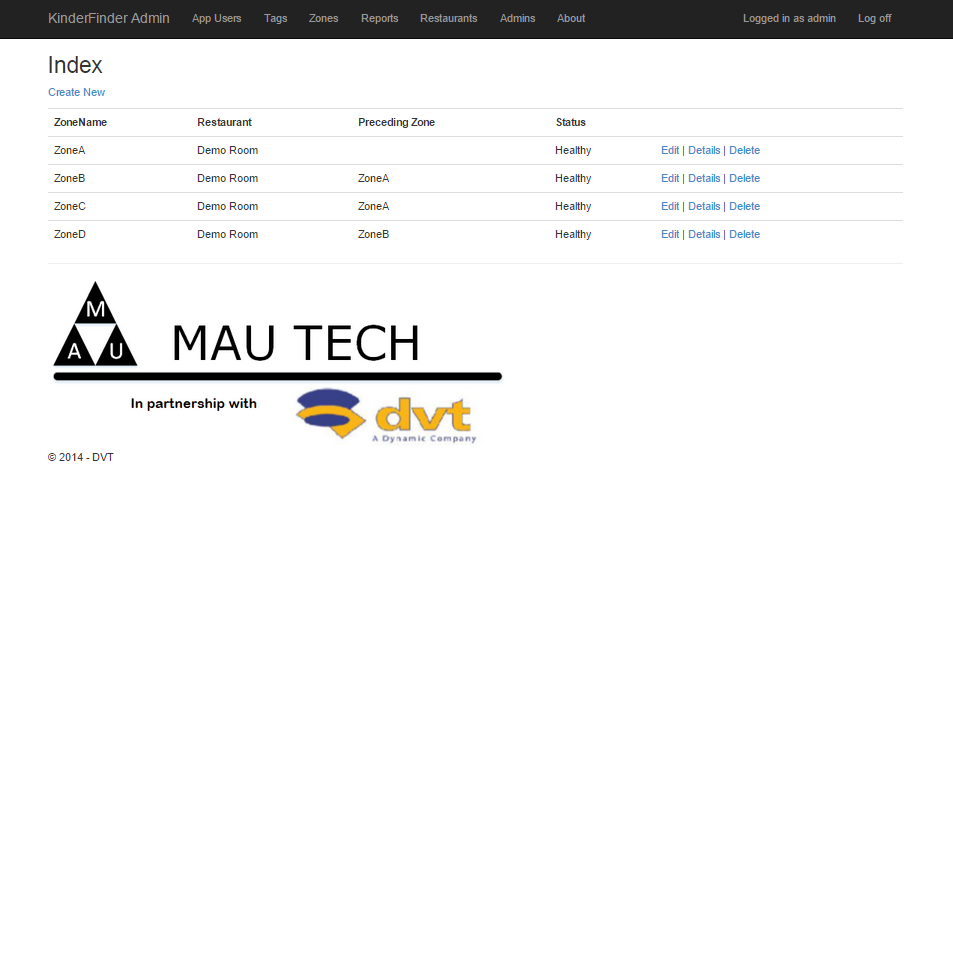
\includegraphics[scale=0.5]{adminportalzones.png}
%\caption{Use case of Android app user (first level granularity).}
%\end{figure}













\end{document}
